\documentclass[twoside,pl,final]{labman}

\usepackage{graphicx}
\usepackage{float}
\usepackage{url}
\usepackage{listings}
\usepackage[caption=false]{subfig}
\usepackage{placeins}

\graphicspath{ {fig/} }

\subject{Projektowanie układów analogowych dla systemów VLSI}
\title{Ekstrakcja parametrów tranzystorów}
\author{mgr inż. Jakub Kopański\\
dr inż. Tomasz Borejko}

\begin{document}
\maketitle
\tableofcontents
\clearpage
\listoffigures
\clearpage
\listoftables
\clearpage

\chapter{Wstęp}
\label{intro}

\section{Motywacja}
\label{intro:motivation}

Rozwój technologii wytwarzania układów scalonych
jest całkowicie podporządkowany względom ekonomicznym.
Znaczna większość sprzedawanych układów to układy całkowicie cyfrowe lub układy,
w których bloki analogowe zajmują niewielką część powierzchni.
Dlatego procesy produkcji układów scalonych są optymalizowane tak,
by uzyskać jak najlepsze parametry układów cyfrowych.

W praktycznie każdym urządzeniu czy systemie do przetwarzania bądź przesyłania
informacji obok układów cyfrowych niezbędne są układy analogowe które
zapewniają łączność, między światem fizycznym,
w którym występują wyłącznie wielkości analogowe, a światem układów cyfrowych.
Począwszy od układów generowania zegara
jakim synchronizowane są współczesne procesory,
przez dokładne przetworniki analogowo/cyfrowe,
warstwy fizyczne magistrali danych takich jak:
\emph{DDR}, \emph{USB} czy \emph{PCIe},
aż po układy do komunikacji bezprzewodowej:
\emph{Bluetooth}, \emph{WiFi}, \emph{GSM}, \emph{LTE}.
Bloki analogowe oraz cyfrowe są często scalane w jednym układzie,
co daje korzyści techniczne i zapewnia minimalny koszt.
Takie układy określane są terminem \emph{System on Chip (SoC)}.
Implementacja bloków analogowych w technologiach CMOS przeznaczonych dla
układów cyfrowych jest jednak dla projektanta tych bloków dużym utrudnieniem.

\section{Cel ćwiczenia}
\label{intro:goal}

W poprzednim rozdziale podane zostało uzasadnienie projektowania
układów analogowych w nowoczesnych technologiach CMOS.
Proste modele matematyczne tranzystorów MOS nie opisują charakterystyk
współcześnie produkowanych tranzystorów z dostateczną dokładnością.
Zaprojektowanie bez nich dobrze działającego
układu scalonego jest praktycznie niemożliwe.
Standardem przemysłowym używanym przy projektowaniu układów scalonych
jest model BSIM4~\cite{bsim4:manual}.
Będzie on również wykorzystywany podczas laboratorium.

Pierwszym etapem projektowania każdego układu
są obliczenia \emph{odręczne}.
Z racji użycia mało dokładnych modeli obarczone są błędem,
ale pozwalają szybko znaleźć dobry punkt startowy do dalszej optymalizacji,
a także odrzucić podejścia z góry skazane na porażkę.
Wyrabiają także umiejętność analizy układów
i zmniejszają liczbę czasochłonnych symulacji.
\emph{Projektantów}, którzy zamiast zrozumieć działanie układów
uruchamiają coraz to nowe symulacje komputerowe w nadziei,
że układ \emph{jakoś zadziała}, określa się żartobliwie mianem
\emph{Spice monkey},~\fig{fig:spicemonkey}

\begin{figure}[!htbp]
  \centering
  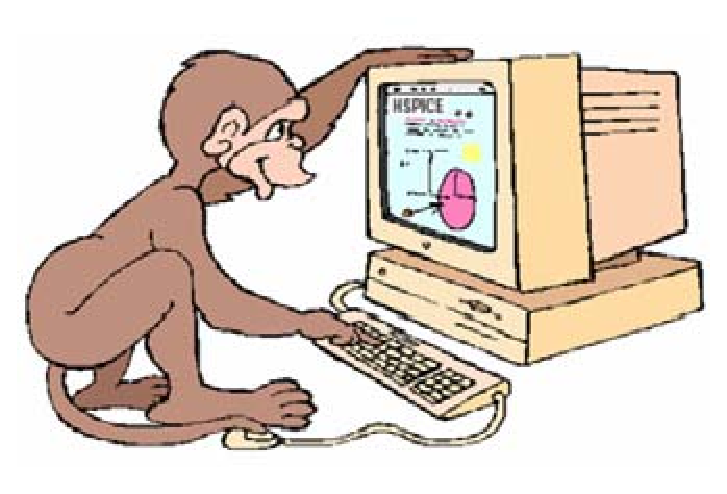
\includegraphics[width=0.4\textwidth]{spicemonkey}
  \caption[\emph{Spice monkey}]{\emph{Spice monkey}. Źródło:~\cite{murmann}}
  \label{fig:spicemonkey}
\end{figure}

Celem ćwiczenia jest zapoznanie studentów z modelami tranzystorów MOS,
użytecznymi w obliczeniach odręcznych,
pokazanie sposobu ekstrakcji parametrów tych modeli
(ze złożonych modeli używanych w symulacjach komputerowych),
a także takie wymiarowanie tranzystorów, aby zapewnić im pożądany punkt pracy.

W trakcie laboratorium przeprowadzone zostaną symulacje tranzystorów wchodzących
w skład nowoczesnej technologii firmy \emph{United Microelectronics Corporation}
o wymiarze charakterystycznym~$130~nm$.
Dla tranzystorów dostępnych w używanej technologii firma \emph{UMC}
dostarcza wartości parametrów modelu BSIM.
Poprzez symulację uzyskane zostaną charakterystyki tranzystorów,
które będą traktowane jak \emph{dane pomiarowe} i posłużą do wyznaczenia
parametrów prostych modeli, nadających się do obliczeń odręcznych.

W ramach laboratorium studenci wykorzystywać będą oprogramowanie
\emph{Virtuoso} firmy \emph{Cadence}.
W celu usprawnienia przebiegu laboratorium, wcześniej przygotowane zostały:
\begin{itemize}
  \item schemat do symulacji,
  \item ustawienia symulatora,
  \item wyrażenia w języku \emph{Skill},
    obliczające parametry prostego modelu na podstawie charakterystyk
    tranzystorów otrzymanych poprzez symulacje komputerową.
\end{itemize}

Wynikiem pracy w laboratorium będzie uzupełniona \tab{tab:devices}.
Wartości uzyskane podczas ćwiczenia i zebrane w tabli~\ref{tab:devices},
posłużą jako punkt startowy projektów realizowanych na kolejnych ćwiczeniach.

\FloatBarrier
\chapter{Model tranzystora MOS}
\label{model}

\section{Model kwadratowy}
\label{model:squarelaw}

\begin{figure}[!htbp]
  \centering
  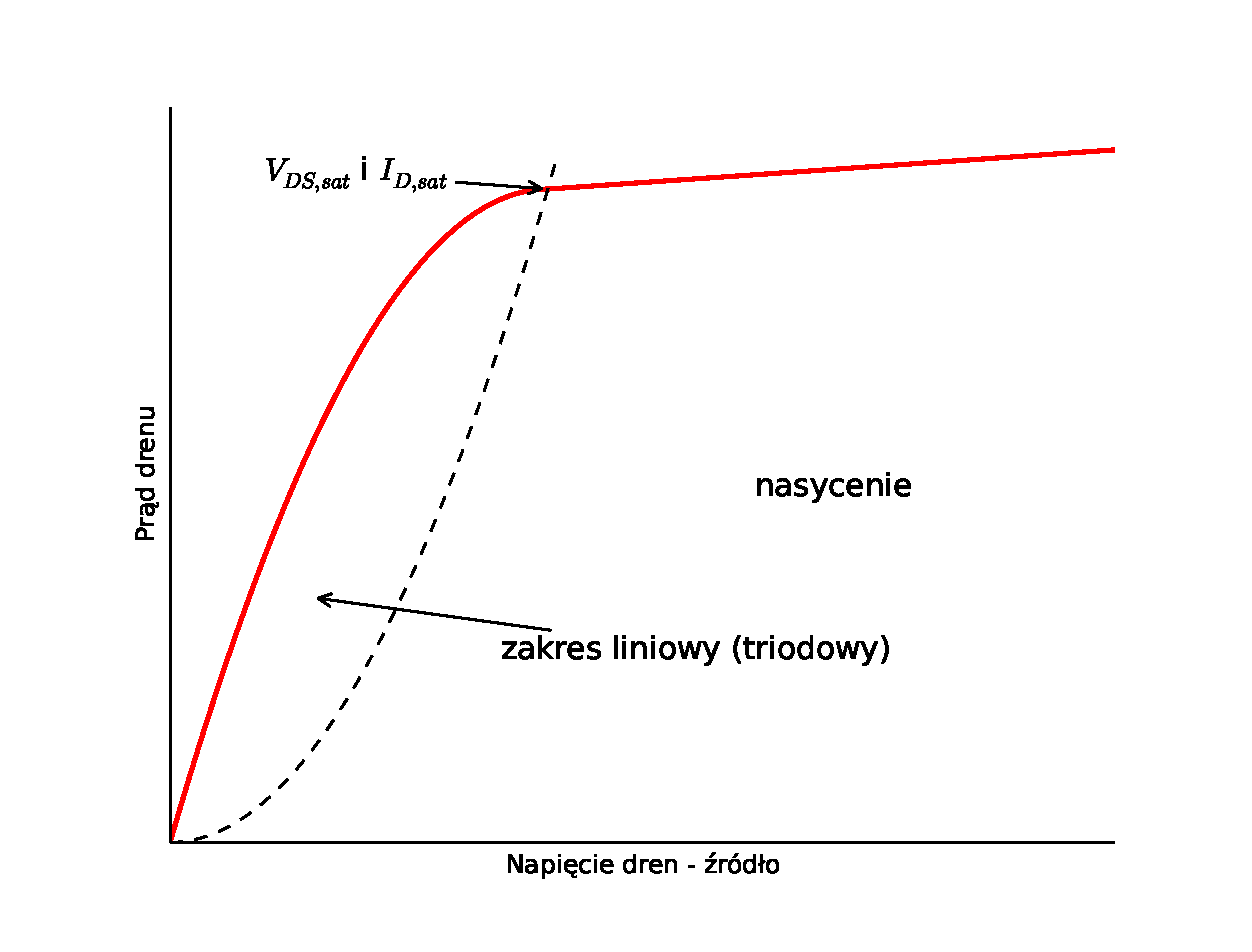
\includegraphics[width=0.9\textwidth]{iv_squarelaw}
  \caption{Charakterystyka modelu tranzystora}
  \label{fig:squarelaw:iv}
\end{figure}

Klasyczne równanie opisujące prąd drenu tranzystora ma postać:
\begin{equation}
  I_D = \mu C_{ox} \cdot \frac{W}{L} \cdot \frac{(V_{GS} - V_{TH}) ^ 2}{2} (1 + \lambda V_{DS})
  \label{eqn:squarelaw:id}
\end{equation}
dla $V_{DS} \geq V_{DSsat}$ i $V_{GS} \geq V_{TH}$,
gdzie $\mu C_{ox}$ oznaczamy~$K_{n,p}$ odpowiednio dla tranzystorów nMOS i pMOS.
Charakterystykę tranzystora opisaną tym równaniem
pokazano na~\fig{fig:squarelaw:iv} $V_{DSsat}$ jest napięciem,
przy którym tranzystor przechodzi
z obszaru liniowego w obszar nasycenia.
Dla przyrządów długo-kanałowych
\eng{long - channel} można zapisać:
\begin{equation}
  V_{DSsat} = V_{GS} - V_{TH}.
  \label{eqn:squarelaw:vdssat}
\end{equation}
Należy zwrócić uwagę, że chociaż wzór~\eqn{eqn:squarelaw:vdssat}
\emph{jest prawdziwy tylko dla przybliżenia długo - kanałowego}
to zarówno dla tranzystorów długo- jak i krótko - kanałowych,
\emph{$V_{DSsat}$ wyznacza granice napięcia $V_{DS}$ pomiędzy
zakresem liniowym a zakresem nasycenia}.
W przypadku granicznym prąd drenu można opisać równaniem:
\begin{equation}
  I_D = K \cdot \frac{W}{L} \cdot \frac{(V_{GS} - V_{TH}) ^ 2}{2} = K \frac{W}{L} \frac{(V_{DSsat}) ^ 2}{2}
  \label{eqn:squarelaw:idsat}
\end{equation}
co pozwala przepisać wzór~\eqn{eqn:squarelaw:id} jako:
\begin{equation}
  I_D = I_{Dsat} + I_{Dsat} \lambda \cdot V_{DS}
  \label{eqn:squarelaw:id:idsat}
\end{equation}

W obszarze nasycenia tranzystor zachowuje się jak źródło prądowe wymuszające
prąd o wartości~$I_{Dsat}$ oraz równolegle połączony rezystor o wartości:
\begin{equation}
  r_{ds} = \frac{1}{\lambda I_{Dsat}}
  \label{eqn:squarelaw:ro}
\end{equation}

\begin{figure}[!htbp]
  \centering
  \includegraphics[]{diode}
  \caption{Tranzystor w połączeniu diodowym}
  \label{fig:diode}
\end{figure}

Na~\fig{fig:diode} pokazano tranzystor, którego bramkę i dren zwarto.
Takie połączenie nazywamy diodowym.
Jest to bardzo często występująca struktura w układach analogowych.
Ponieważ $V_{GS} = V_{DS}$, to przy~$V_{GS} \geq V_{TH}$
(jeżeli przez tranzystor będzie płynął prąd),
aby tranzystor pracował w nasyceniu musi być spełniony warunek:~$V_{DS} \geq V_{GS} - V_{TH}$,
co daje:~$0 \geq -V_{TH}$.
Wynik ten mówi, że tranzystor w połączeniu diodowym
jest \emph{zawsze} w nasyceniu.

\FloatBarrier
\section{Właściwości modelu \emph{kwadratowego}}
\subsection{Transkonduktancja $g_m$}
\label{model:squarelaw:gm}

\begin{figure}[!htbp]
  \centering
  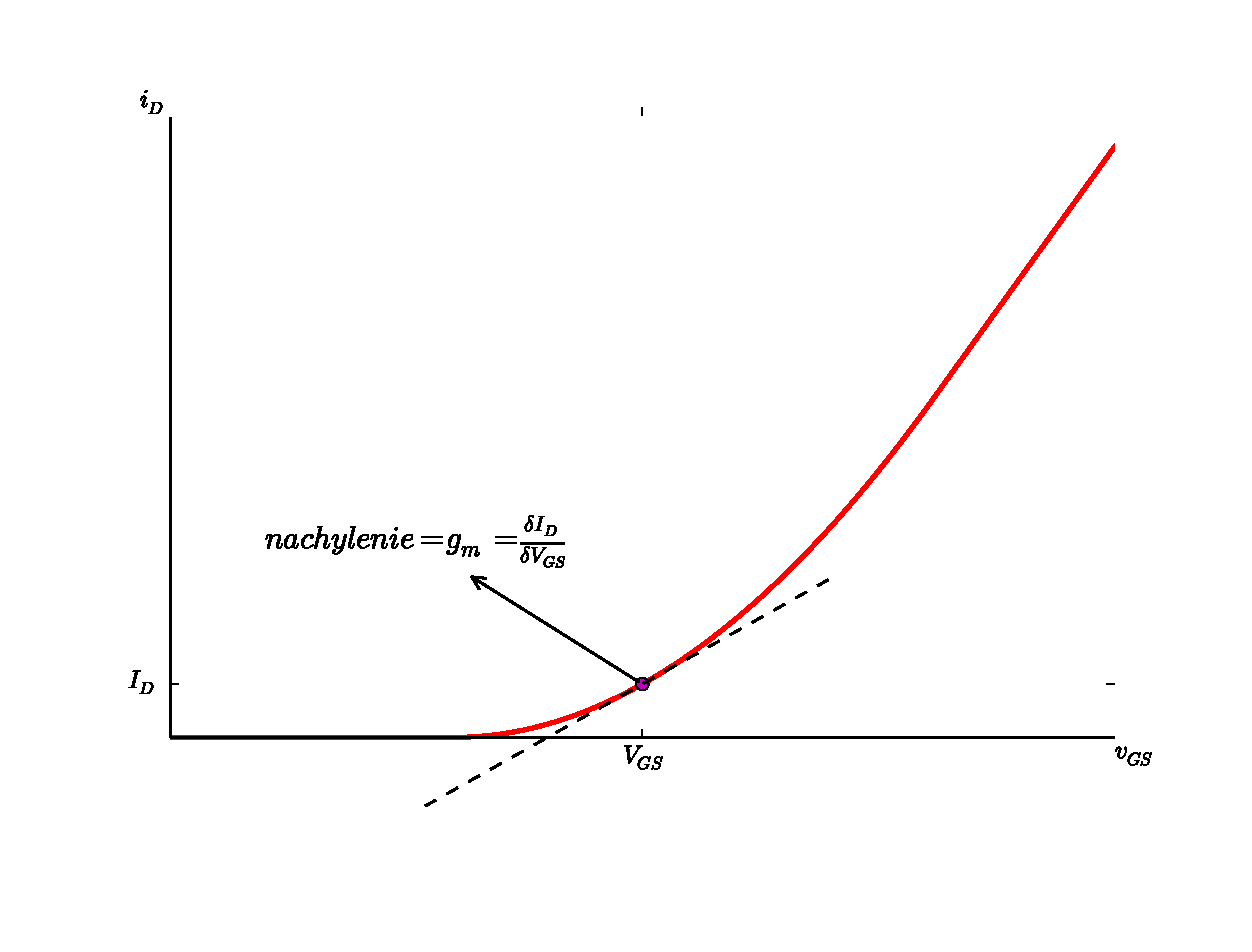
\includegraphics[width=0.9\textwidth]{gm}
  \caption{Wyznaczanie transkonduktancji}
  \label{fig:squarelaw:gm}
\end{figure}

Jednym z najważniejszych parametrów tranzystora,
używanym przy projektowaniu układów analogowych,
jest transkonduktancja.
Jest ona pochodną prądu drenu po napięciu bramka - źródło.
\begin{equation}
  g_m = \frac{\delta I_D}{\delta V_{GS}} \Bigg\vert_{V_{DS} = const}
  \label{eqn:squarelaw:gm:deriv}
\end{equation}

Małosygnałowa składowa prądu drenu~$i_d$ wiąże się z małosygnałową składową
napięcia bramki~$v_{gs}$ zależnością:
\begin{equation}
  i_d = g_m \times v_{gs},
  \label{eqn:squarelaw:trans}
\end{equation}
gdzie  $|v_{gs}| \ll V_{GS}$ i $|i_d| \ll I_D$.

Różniczkując~\eqn{eqn:squarelaw:id} otrzymujemy:
\begin{equation}
  g_m = \beta (V_{GS} - V_{TH}) = \sqrt{2 \beta I_D} = \frac{2 I_D}{V_{GS} - V_{TH}},
  \label{eqn:squarelaw:gm}
\end{equation}
gdzie $\beta = K \frac{W}{L}$.
Warto zauważyć, że wartość transkonduktancji (w zakresie nasycenia)
rośnie proporcjonalnie do napięcia~$V_{GS}$ oraz
proporcjonalnie do pierwiastka prądu drenu.

Transkonduktancję można wyznaczyć z charakterystyki przejściowej tranzystora.
Wartość transkonduktancji jest równa nachyleniu stycznej
do wykresu prądu drenu w funkcji napięcia bramka - źródło w punkcie pracy.
Ten sposób wyznaczania transkonduktancji zaprezentowano na~\fig{fig:squarelaw:gm}

\FloatBarrier
\subsection{Rezystancja wyjściowa $r_{ds}$}
\label{model:squarelaw:ro}

\begin{figure}[!htbp]
  \centering
  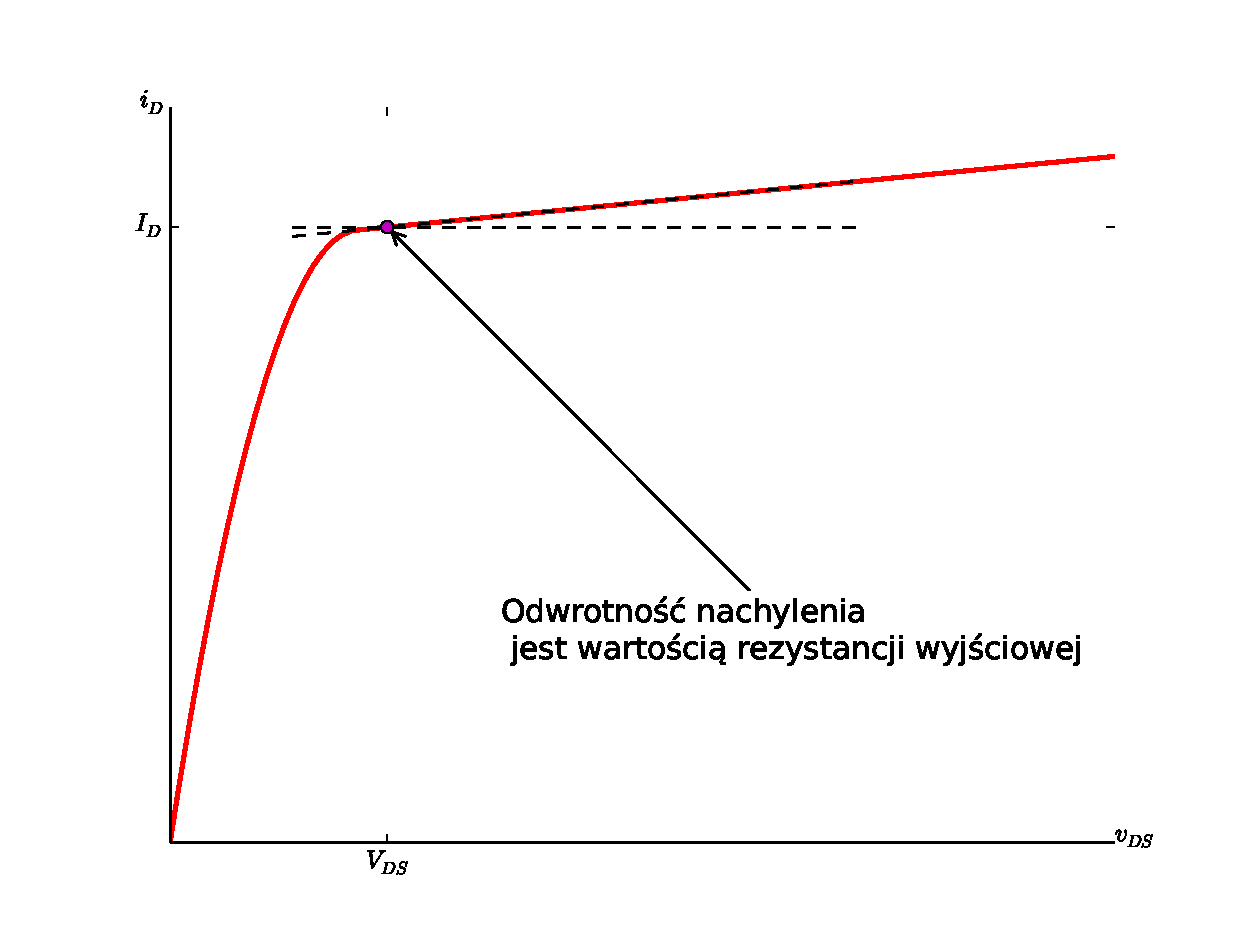
\includegraphics[width=0.9\textwidth]{ro}
  \caption{Wyznaczanie rezystancji wyjściowej}
  \label{fig:squarelaw:ro}
\end{figure}

Wzór~\eqn{eqn:squarelaw:ro} nieformalnie określa rezystancję
wyjściową w nasyceniu dla modelu kwadratowego.
Formalnie rezystancja wyjściowa jest odwrotnością konduktancji wyjściowej:
\begin{equation}
  r_{ds} ^ {-1} = g_{ds} = \frac{\delta I_D}{\delta V_{DS}} \Bigg\vert_{V_{GS} = const}
  \label{eqn:ro:deriv}
\end{equation}
Co po zróżniczkowaniu~\eqn{eqn:squarelaw:id} daje ten sam wynik, co~\eqn{eqn:squarelaw:ro}.

Jeżeli wyznaczymy~$r_{ds}$, to~$\lambda$ możemy obliczyć jako:
\begin{equation}
  \lambda = \frac{1}{I_{Dsat} \cdot r_{ds}}
  \label{eqn:ro:lambda}
\end{equation}

Parametr~$\lambda$ ma tym większą wartość, im krótszy jest kanał tranzystora,
w pierwszym przybliżeniu można przyjąć, że~$\lambda \varpropto \frac{1}{L}$.
Wówczas z~\eqn{eqn:squarelaw:ro} wynika, że:
\begin{equation}
  r_o \varpropto \frac{L^2}{V_{DSsat}^2}
  \label{eqn:ro:prop}
\end{equation}
Z zależności~\eqn{eqn:ro:prop} możemy wnioskować,
że dla stałego napięcia~$V_{GS}$,
gdy zwiększamy długość kanału to rezystancja wyjściowa rośnie.
Przy zachowaniu stałej długości kanału rezystancje wyjściową można zwiększyć
zmniejszając~$V_{DSsat}$.
Warto zauważyć, że efektem ubocznym takich działań będzie zmniejszenie prądu drenu.
Zobaczymy dalej, że w układach analogowych korzystne jest,
aby rezystancja wyjściowa była jak największa.
Skłania to do projektowania tranzystorów z długimi kanałami
ale --- jak zobaczymy --- takie podejście ma również swoje wady.

Rezystancje wyjściową można wyznaczyć również graficznie,
co pokazano na~\fig{fig:squarelaw:ro}
Jest ona równa odwrotności nachylenia charakterystyki
prądu drenu w zakresie nasycenia.

\FloatBarrier
\subsection{Napięcie progowe $V_{TH}$}
\label{model:squarelaw:vth}

\begin{figure}[!htbp]
  \centering
  \subfloat[Na podstawie charakterystyki przejściowej\label{fig:vth:id}]{
    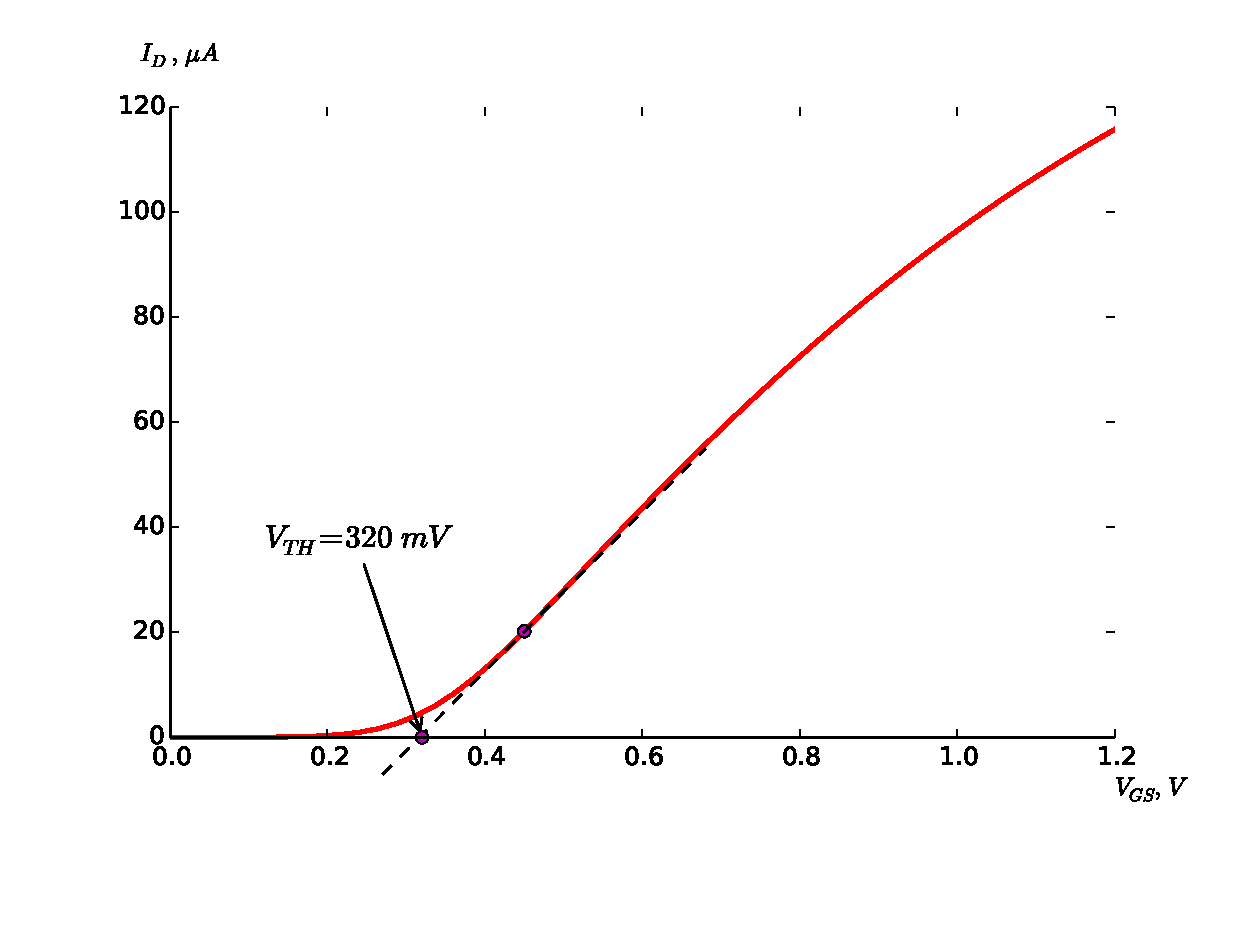
\includegraphics[width=0.48\textwidth]{vth_id}
  }
  \hfill
  \subfloat[Na podstawie charakterystyki transkonduktancji w funkcji napięcia branka-źródło\label{fig:vth:gm}]{
    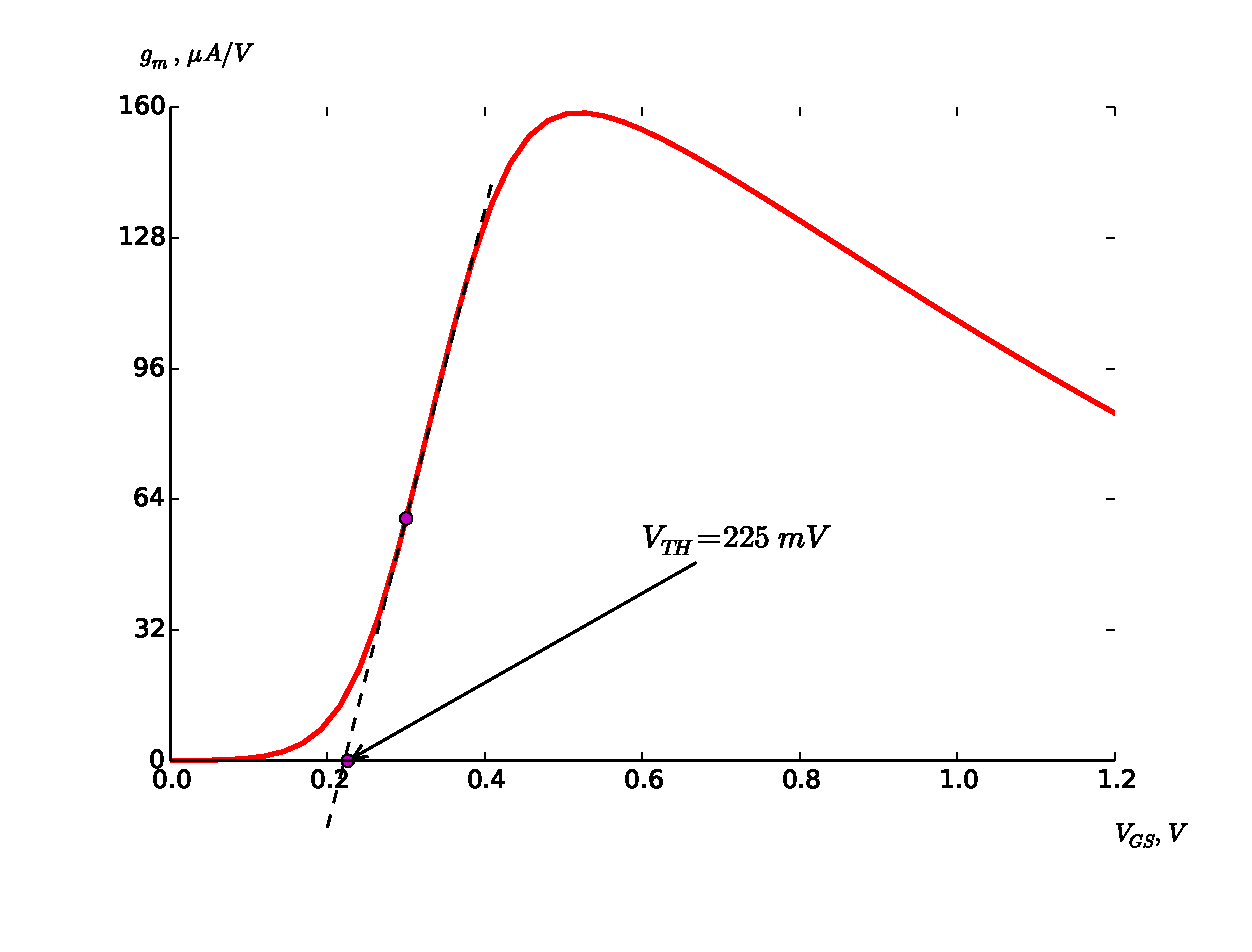
\includegraphics[width=0.48\textwidth]{vth_gm}
  }
  \caption{Sposoby wyznaczania napięcia progowego}
  \label{fig:vth}
\end{figure}

Kolejnym istotnym parametrem jest napięcie progowe tranzystora.
Parametr ten nie ma jednoznacznej, ścisłej definicji,
jego wartość można więc wyznaczyć rozmaicie w zależności od tego,
do jakich obliczeń jest ta wartość potrzebna.
Typowo można wyznaczyć je korzystając z charakterystyki przejściowej
tranzystora z~\fig{fig:squarelaw:gm}
Napięcie progowe jest równe wartości napięcia $V_{GS}$,
dla którego styczna z~\fig{fig:squarelaw:gm} przecina się z osią odciętych.
Metoda ta jest dobra dla tranzystora pracującego w stanie silnej inwersji,
gdy~$V_{GS} \gg V_{TH}$.
W przypadku podobnym jak na~\fig{fig:squarelaw:gm},
gdy napięcie bramka-źródło jest tylko nieznacznie większe od napięcia progowego,
trudno jest wyznaczyć styczną,
przez co również trudno jest określić napięcie progowe.
Wyznaczanie napięcia progowego dodatkowo może skomplikować praca z napięciem
dren-źródło tylko nieznacznie większym od napięcia nasycenia~$V_{DSsat}$.
W takim przypadku charakterystyka przejściowa ma kształt zaprezentowany na~\fig{fig:vth:id},
który odbiega od wcześniej prezentowanego przebiegu z~\fig{fig:squarelaw:gm}

W innej metodzie wykorzystuję się liniową zależność tanskonduktancji
od napięcia bramka-źródło~$g_m = \beta( V_{GS} - V_{TH})$.
Potrzebna charakterystyka widoczna jest na~\fig{fig:vth:gm}.
Uzyskuje się ją poprzez obliczenie pochodnej prądu drenu po napięciu~$V_{GS}$.
Na wykresie prowadzi się styczną z zakresu
liniowej zależności transkonduktancji od~$V_{GS}$.
Napięcie~$V_{GS}$, dla którego styczna przecina oś odciętych
jest napięciem progowym~$V_{TH}$, zgodnie ze wzorem~\eqn{eqn:squarelaw:gm}.

Obie metody dają różne wyniki.
Ze względu na to, że przewidujemy prace tranzystora w pośredniej inwersji,
przy małym zapasie napięcia dren-źródło ponad napięcie nasycenia,
zastosujemy metodę z~\fig{fig:vth:gm}

\FloatBarrier
\subsection{Częstotliwość graniczna tranzystora $f_T$}
\label{model:squarelaw:ft}

\begin{figure}[!htbp]
  \centering
  \includegraphics[height=0.25\textheight]{ft_measure}
  \caption{Pomiar częstotliwości granicznej $f_T$}
  \label{fig:ft:meas}
\end{figure}

Na~\fig{fig:ft:meas} zaprezentowano układ do pomiaru
częstotliwości granicznej tranzystora~$f_T$.
Dla sygnału dren tranzystora jest zwarty (przez źródło DC) do masy.
Dzięki temu pojemności~$C_{gd}$~i~$C_{gs}$, dla sygnału, są połączone równolegle.
Można zatem zapisać:
\begin{equation}
  v_{gs} = \frac{i_g}{\jmath \omega \cdot (C_{gs} + C_{gd})}
  \label{eqn:ft:vgs}
\end{equation}
Ponieważ, jak wiemy ze wzoru~\eqn{eqn:squarelaw:trans}:~$i_d = g_m \times v_{gs}$,
możemy zapisać:
\begin{equation}
  \Big \vert \frac{i_d}{i_g} \Big \vert = \frac{gm}{2 \pi f \cdot (C_{gs} + C_{gd})}
  \label{eqn:ft:igain}
\end{equation}

Częstotliwością graniczną tranzystora~$f_T$ nazywamy częstotliwość sygnału
dla którego wzmocnienie prądowe, spada do wartości~$1$.
Wzmocnienie prądowe ma sens tylko dla sygnału wielkiej częstotliwości.
Prąd wejściowy~$i_g$ istnieje z powodu występowania
pojemności zaznaczonych na~\fig{fig:ft:meas}

Uwzględniając, że $C_{gs} \gg C_{gd}$,
można zapisać:
\begin{equation}
  f_T \approx \frac{gm}{2 \pi f C_{gs}}
            = \frac{3 KP \cdot (V_{GS} - V_{TH})}{4 \pi \cdot L^2 C_{ox}^{\prime}}
            = \frac{3 \mu}{4 \pi} \cdot \frac{V_{DS,sat}}{L^2}
  \label{eqn:ft:ft}
\end{equation}
W stanie nasycenia przyblizona wartość
pojemności~$C_{gs}$ wynosi~$\frac{2}{3} W L C_{ox}^{\prime}$.

Wnioski płynące ze wzoru~\eqn{eqn:ft:ft} są bardzo istotne.
Projektując układy przeznaczone do pracy przy wielkich częstotliwościach,
należy używać tranzystorów o minimalnych długościach kanałów
oraz pracujących przy wysokim napięciu nasycenia~$V_{DS,sat}$.
Jednak tranzystory z krótkim kanałem mają małą wartość rezystancji wyjściowej
(patrz punkt~\ref{model:squarelaw:ro}), czego konsekwencją jest
--- jak zobaczymy później --- mała wartość wzmocnienia napięciowego.
Z kolei duża wartość napięcia nasycenia utrudnia uzyskanie dużej amplitudy
napięcia na wyjściu wzmacniacza.

\FloatBarrier
\section{Model tranzystora z \emph{krótkim kanałem}}
\label{model:short}

W niniejszym rozdziale zostaną przedstawione odstępstwa od poprzedniego modelu
wprowadzone aby uchwycić efekty \emph{krótkiego kanału}
\eng{short-channel effetcs} jakie występują w nowoczesnych technologiach
o małym wymiarze charakterystycznym.

\subsection{Napięcie nasycenia $V_{DS,sat}$}
\label{model:short:vdssat}

Bardzo ważny wzór~\eqn{eqn:squarelaw:vdssat} określający napięcie nasycenia
tranzystora \emph{nie ma zastosowania} dla tranzystorów z krótkim kanałem,
ponieważ model kwadratowy nie opisuje z dostateczną dokładnością ich charakterystyk.
Różnica pomiędzy napięciem bramka-źródło, a napięciem progowym,
w przypadku tranzystora krótko-kanałowego,
jest nazywana napięciem \emph{przesterowania} \eng{overdrive}.
Termin \emph{przesterowanie} w języku polskim jest używany w trochę innym znaczeniu,
jednak autor niniejszej instrukcji nie spotkał się,
z polskim tłumaczeniem, które dobrze oddawałoby charakter
nadmiaru napięcia~$V_{GS}$ nad~$V_{TH}$.
Podsumowując, w przypadku tranzystora krótko-kanałowego:
\begin{equation}
  V_{ov} = V_{GS} - V_{TH} \neq V_{DSsat}
  \label{eqn:short:vov}
\end{equation}

\subsection{Częstotliwość graniczna tranzystora $f_T$}
\label{model:short:ft}

Dla tranzystorów krótko-kanałowych ruchliwość nośników nie jest stała,
ale maleje przy zmniejszaniu długości kanału.
Jest to efekt nasycenia prędkości nośników,
spowodowany większym polem elektrycznym w kanale.
Z tego względu we wzorze~\eqn{eqn:ft:ft} składnik~$\frac{\mu}{L}$
można potraktować jako stały i zapisać
\begin{equation}
  f_t \approx \frac{g_m}{2 \pi C_{gs}} \varpropto \frac{V_{ov}}{L}
  \label{eqn:short:ft}
\end{equation}

Wnioski pozostają podobne jak w rozdziale~\ref{model:squarelaw:ft}.
Gdy zależy nam na pracy tranzystora w zakresie wysokich częstotliwości,
należy używać większych wartości napięcia~$V_{ov}$,
kosztem zmniejszonego zakresu napięcia sygnału na wyjściu wzmacniacza.

\subsection{Prąd drenu i transkonduktancja $g_m$}
\label{model:short:id_gm}

Dla tranzystora krótko-kanałowego prąd drenu ma postać~\cite{baker:book}:
\begin{equation}
  I_D = W \cdot \nu_{sat} \cdot C_{ox}^\prime (V_{GS} - V_{TH} - V_{DSsat})
  \label{eqn:short:id}
\end{equation}
Transkonduktancję można wyznaczyć
tak jak poprzednio we wzorze~\eqn{eqn:squarelaw:gm:deriv}:
\begin{equation}
  g_m = \frac{\delta I_D}{\delta V_{GS}} \Bigg\vert_{V_{DS} = const}
      = \frac{\delta}{\delta V_{GS}}\big(W \cdot \nu_{sat} \cdot C_{ox}^\prime (V_{GS} - V_{TH} - V_{DSsat})\big)
      = \nu_{sat} \cdot C_{ox}^\prime \cdot W
  \label{eqn:short:gm}
\end{equation}
Transkonduktancja tranzystora krótko-kanałowego
w pierwszym przybliżeniu zależy tylko od szerokości kanału
(gdy dojdzie do nasycenia prędkości nośników).
Jednak w rzeczywistości instnieją inne bardziej skomplikowane efekty fizyczne,
które sprawiają,
\emph{że $g_m$ rośnie wraz ze wzrostem napięcia $V_{GS}$ lub $V_{DS}$}.

\subsection{Rezystancja wyjściowa $r_{ds}$}
\label{model:short:ro}

\begin{figure}[!htbp]
  \centering
  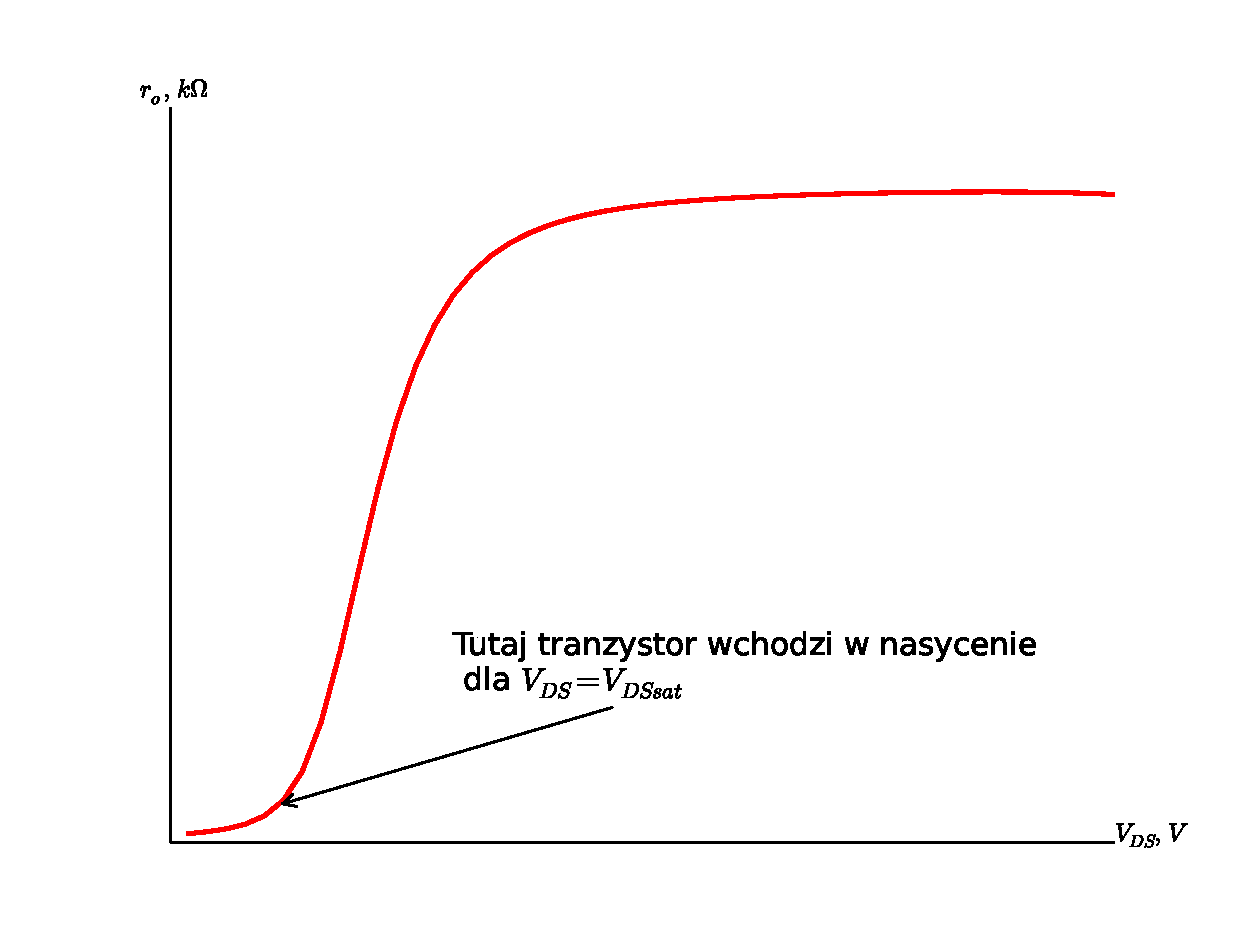
\includegraphics[width=0.9\textwidth]{short_ro}
  \caption{Rezystancji wyjściowa tranzystora z krótkim kanałem}
  \label{fig:short:ro}
\end{figure}

Rezystancję wyjściową wyznaczamy podobnie jak w przypadku tranzystora z długim
kanałem biorąc odwrotność pochodnej prądu drenu po napięciu dren-źródło.
Charakterystykę rezystancji wyjściowej w funkcji
napięcia dren-źródło zaprezentowano na~\fig{fig:short:ro}

Ten sam wykres służy również do orientacyjnego wyznaczenia napięcia nasycenia.
Wartość napięcia~$V_{DS}$, poczynając od której rezystancja wyjściowa zaczyna
\emph{gwałtownie} rosnąć, możemy uważać za napięcie nasycenia~$V_{DSsat}$.
Warto zwrócić uwagę, że używając większych wartości napięcia~$V_{DS}$
można uzyskać znacznie większą rezystancje wyjściową.
To ważne spostrzeżenie, do którego powrócimy w kolejnym
ćwiczeniu przy projektowaniu luster prądowych.

\FloatBarrier
\chapter{Wymiarowanie i polaryzacja tranzystorów}
\label{sizing}

\section{Parametry modeli}
\label{sizing:params}

W rozdziale~\ref{model} przedstawione zostały przybliżone modele tranzystorów.
Są one niezbędne przy projektowaniu i analizie układów elektronicznych.
Producent układów dostarcza jedynie wartości parametrów modelu~BSIM,
lub innego podobnie złożonego, dobranego doświadczalnie tak,
by jak najdokładniej opisać charakterystyki tranzystorów produkowanych w danej technologii.
Wartości parametrów modelu bardziej złożonego nie mogą być użyte w modelu prostszym.
W ćwiczeniu nauczymy się określać wartości parametrów prostego modelu na
podstawie modelu dostarczanego przez producenta układów.

Pokazany w ćwiczeniu sposób określenia parametrów modelu
opisany jest w literaturze, poz.~\cite{baker:book}, rozdział 9.

\section{Długość kanału tranzystora}
\label{sizing:l}

Bazując na tym co zostało powiedziane w rozdziale~\ref{model} można
napisać kilka ogólnych porad na temat wymiarowania tranzystorów.
Typowo w projektach analogowych staramy się nie używać
minimalnych długości kanału tranzystora
(dokładnie rzecz ujmując, minimalnych wymiarów w ogóle).
Na potrzeby ćwiczenia wartością, od jakiej można zacząć projekt
jest długość kanału od~2 do~5 razy większa niż minimalna możliwa.

\section{Napięcie nasycenia $V_{DSsat}$ i $V_{ov}$}
\label{sizing:vdssat}

W celu wykonania ćwiczenia należy przyjąć początkową
wartość napięcia $V_{DSsat}$ i $V_{ov}$.
W pierwszym przybliżeniu można przyjąć wartość równą
$5\%$~napięcia zasilania~$V_{dd}$,
co dla technologii używanej na zajęciach,
daje wartość równą~$5\% \ 1,2~V = 60~mV$.
Jest to przybliżone oszacowanie napięcia~$V_{ov}$ i często modyfikuje się
uzyskany wynik tak, by po dodaniu do~$V_{TH}$ dawał
\emph{okrągłą} wartość napięcia~$V_{GS}$.

\section{Szerokość kanału $W$}
\label{sizing:w}

Wybór szerokości kanału przy ustalonych w poprzednich punktach napięciach
i wymiarach podyktowany jest pożądaną wartością prądu drenu w punkcie pracy.
W ramach ćwiczeń można przyjąć, że prąd drenu tranzystora,
jaki chcemy uzyskać w punkcie pracy,
wynosi~$10~\mu{}A$.

\chapter{Określenie parametrów tranzystorów}
\label{measure}

\section{Praca w środowisku \emph{Virtuoso}}
\label{measure:virtuoso}

\subsection{Uruchomienie}
\label{measure:virtuoso:run}

Konfiguracja, uruchomienie oraz podstawy użytkowania środowiska
\emph{Cadence Virtuoso} opisano w osobnym dokumencie~\cite{adec:cds:man}.

Podczas ćwiczenia 1 będziemy korzystać z komórki \emph{baker\_sim}
z biblioteki \emph{LAB1}.

\begin{figure}[!htbp]
  \centering
  \includegraphics[width=0.9\textwidth]{baker_sch}
  \caption{Edytor schematu i uruchomienie ustawień symulacji}
  \label{fig:measure:baker_sch}
\end{figure}

Na~\fig{fig:measure:baker_sch} pokazano edytor schematu z komórką baker\_sim.
Aby możliwa byłą symulacja układu,
należy jeszcze otworzyć ustawienia symulacji.
W tym celu, w oknie edytora schematu należy wybrać \emph{Launch -> ADE GXL},
co pokazano na~\fig{fig:measure:baker_sch}
W oknie jakie się pojawi należy zaznaczyć opcje \emph{Open existing cellview}
i wcisnąć \emph{OK}.
W kolejnym nowo otwartym oknie należy wybrać odpowiedni \emph{View},
jak ilustruje~\fig{fig:measure:adexl_open}.

\begin{figure}[!htbp]
  \centering
  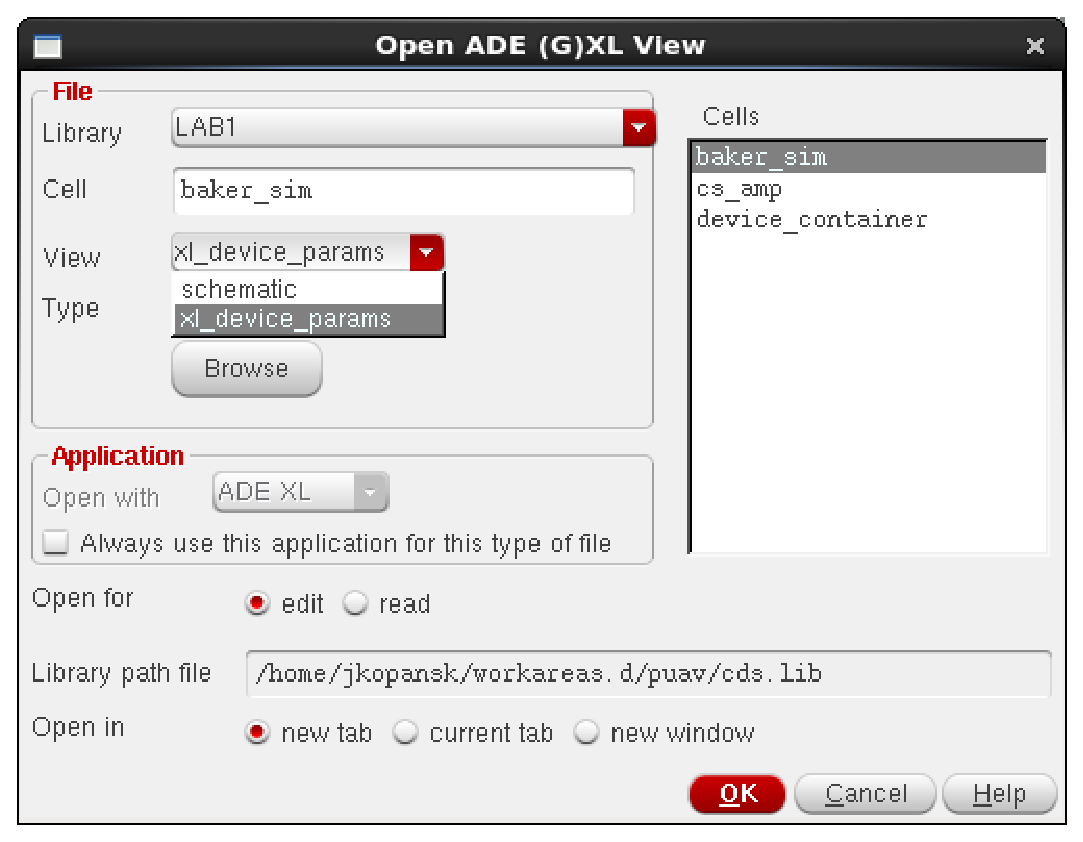
\includegraphics[width=0.9\textwidth]{adexl_open}
  \caption{Otwarcie przygotowanych wcześniej ustawień symulacji}
  \label{fig:measure:adexl_open}
\end{figure}

\subsection{Obsługa symulatora}
\label{measure:virtuoso:sim}

\begin{figure}[!htbp]
  \centering
  \includegraphics[angle=90,width=0.9\textwidth]{baker_adexl}
  \caption{Ustawienia symulacji}
  \label{fig:measure:baker_adexl}
\end{figure}

Na~\fig{fig:measure:baker_adexl} pokazano okno przygotowania symulacji
wraz z zaznaczonymi kluczowymi elementami.
Praca z układem na ćwiczeniu polega na modyfikowaniu zmiennych parametrów symulacji,
parametrów tranzystorów, a następnie weryfikowaniu wyników symulacji.

W tabeli~\ref{tab:measure:sims} zebrane zostały predefiniowane symulacje,
oraz jakie parametry są wyznaczane z charakterystyk uzyskanych w danej symulacji.

Napięcie progowe wyznaczane jest tak,
jak zostało to zaprezentowane na~\fig{fig:vth:gm}
Charakterystykę transkonduktancji w funkcji napięcia bramka-źródło,
niezbędną do wyznaczenia napięcia progowego,
otrzymuje się korzystając z wbudowanej w środowisko
\emph{Virtuoso} funkcji różniczkowania.

Wartość transkonduktancji jest odczytywana z otrzymanego wcześniej przebiegu
dla napięcia~$V_{GS} = vth(n/p) + vov(n/p)$,
gdzie $vth(n/p)$ i $vov(n/p)$ to zmienne opisane w tabeli~\ref{tab:measure:vars}.

Aby wyznaczyć rezystancje wyjściową, różniczkuję się charakterystykę wyjściową,
a następnie oblicza się odwrotność pochodnej,
zgodnie z definicją podaną przez wzór~\eqn{eqn:ro:deriv}.
Wartość rezystancji wyjściowej, jaka jest zwracana w oknie wyników,
jest wartością dla wyznaczonego wcześniej prądu drenu.

Wartość~$I_D$ jaką można zobaczyć w oknie wyników,
jest wartością dla napięcia dren-źródło równego $Vds(n/p)$.

Wynik~$Vds(n/p)$ to wartość napięcia dren-źródło,
dla którego tranzystor powinien być w nasyceniu z pewnym zapasem.
Jest to napięcie dren - źródło, dla którego rezystancja wyjściowa
\emph{rośnie} najszybciej,
czyli wartość pochodnej~$r_{ds}$ po napięciu~$V_{DS}$ jest największa.

Częstotliwość graniczna~$f_T$ tranzystora wyznaczona jest z definicji,
tzn.~jest to częstotliwość dla której wzmocnienie prądowe,
określone wzórem~\eqn{eqn:ft:igain}, osiąga wartość 1.
Jedyna różnica to taka, że w symulacji możliwy jest bezpośredni dostęp do
prądów:~$i_g$ oraz~$i_d$.

\begin{table}[htbp]
  \centering
  \caption{Analizy}
  \label{tab:measure:sims}
  \begin{tabular}{l l p{0.7\textwidth}}
    \hline \hline
    Test & Wyznaczane parametry & Opis \\
    \hline
    Vthn & $V_{THN}$, $g_{mn}$ & symulacja określająca charakterystykę przejściową $I_D(V_{GS})$ przy stałym $V_{DS}$ równym wartości zmiennej vdsatn \\
    Vthp & $V_{THP}$, $g_{mp}$ & symulacja określająca charakterystykę przejściową $I_D(V_{GS})$ przy stałym $V_{DS}$ równym wartości zmiennej vdsatp \\
    ron  & $I_D$, $r_o$, $V_{DS,sat}$ & symulacja określająca charakterystykę wyjściową $I_D(V_{DS})$ przy stałym $V_{GS}$ równym Vthn + Vovn \\
    rop  & $I_D$, $r_o$, $V_{DS,sat}$ & symulacja określająca charakterystykę wyjściową $I_D(V_{DS})$ przy stałym $V_{GS}$ równym Vthp + Vovp \\
    fT   & $f_T$ & symulacja określająca częstotliwość graniczną tranzystora \\
    \hline \hline
  \end{tabular}
\end{table}

\begin{table}[htbp]
  \centering
  \caption{Zmienne do ustawień symulacji}
  \label{tab:measure:vars}
  \begin{tabular}{l l}
    \hline \hline
    Zmienna & Opis \\
    \hline
    Vsbn   & napięcie źródło - podłoże tranzystora typu N \\
    Vsbp   & napięcie źródło - podłoże tranzystora typu P \\
    Vdd    & napięcie zasilania \\
    Vthn   & napięcie progowe tranzystora typu N \\
    Vovn   & napięcie \emph{overdrive} tranzystora typu N \\
    Vthp   & napięcie progowe tranzystora typu P \\
    Vovp   & napięcie \emph{overdrive} tranzystora typu P \\
    vdsatn & napięcie $V_{DS}$ tranzystora typu N przy której wykonywane są symulacje \\
    vdsatp & napięcie $V_{DS}$ tranzystora typu N przy której wykonywane są symulacje \\
    \hline \hline
  \end{tabular}
\end{table}

\appendix
\chapter{Parametry tranzystorów}
\label{app:devices}

Tabela z parametrami tranzystorów oraz z miejscami do uzupełnienia.
Wypełniona tabela stanowi wynik ćwiczenia,
podpisaną należy oddać prowadzącemu.
Należy zachować wypełnioną kopie,
ponieważ wyniki będą potrzebne na kolejnych laboratoriach.

\begin{table}[htbp]
  \centering
  \caption{Parametry tranzystorów}
  \label{tab:devices}
  \begin{tabular}{ || c | c | c | p{0.4\textwidth} || }
    \hline \hline
    Parameter & nmos & pmos & Komentarz \\
    \hline
    Prąd polaryzacji, $I_D$ & $10~\mu{}A$ & $10~\mu{}A$ & Wartość przybliżona \\ \hline
    L                       &             &             &                                              \\ \hline
    WF                      &             &             & Szerokość pojedynczego \emph{palca}          \\ \hline
    nf                      &             &             & Liczba \emph{palców}                         \\ \hline
    m                       &             &             & Mnożnik równoległych tranzystorów  \\ \hline
    WT                      &             &             & Całkowita szerokość: $WF \times nf \times m$ \\ \hline
    $V_{DS,sat}$            &             &             & \\ \hline
    $V_{DS}$                &             &             & Wybrany punkt pracy \\ \hline
    $V_{ov}$                &             &             & \\ \hline
    $V_{GS}$                &             &             & \\ \hline
    $V_{TH}$                &             &             & \\ \hline
    $\nu_{sat}$             & $95 \times 10^3 \frac{m}{s}$ & $117 \times 10^3 \frac{m}{s}$ & Z parametrów modelu BSIM \\ \hline
    $t_{ox}$                & $2.73~nm$ & $2.86~nm$ & $toxe$ z parametrów modelu BSIM \\ \hline
    $\epsilon_{ox}$         & $3.9$ & $3.9$ & $epsrox$ z parametrów modelu BSIM \\ \hline
    $C_{ox}^\prime = \frac{\epsilon_{ox}}{t_{ox}}$ & & & \\ \hline
    $C_{ox}$                & & & $C_{ox} = C_{ox}^\prime \times WT \times L$ \\ \hline
    $C_{gs}$                & & & $C_{gs} = \frac{2}{3} \times C_{ox}$ \\ \hline
    $CGDO$                  & $290~pF$ & $310~pF$ & \\ \hline
    $C_{gd}$                & & & $C_{gd} = CGDO \times W$ \\ \hline
    $g_{m}$                 &             &             & Dla $I_D = 10~\mu{}A$ \\ \hline
    $r_{o}$                 &             &             & Dla $I_D = 10~\mu{}A$ \\ \hline
    $g_mr_o$                &             &             & Wzmocnienie bez obciążenia \\ \hline
    $f_T$                   &             &             & \\
    \hline \hline
  \end{tabular}
\end{table}

\bibliographystyle{IEEEtran}
\bibliography{IEEEabrv,bibliography}

\end{document}
